\chapter*{ANDROID: LA REVOLUCIÓN MÓVIL}

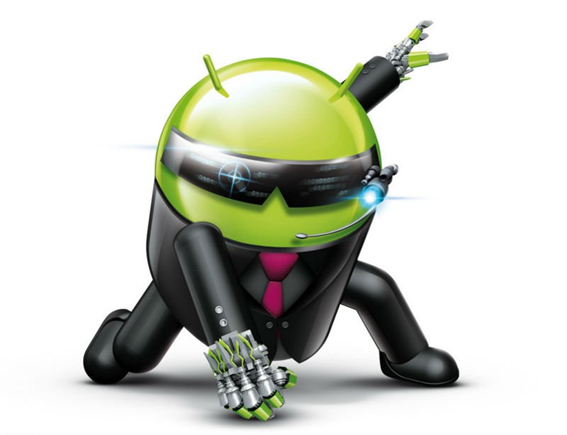
\includegraphics[scale=0.7]{img/cp05/img0501.png}

Android es un sistema operativo de código abierto basado en Linux, utilizado en dispositivos móviles con pantalla táctil como Smartphones y Tablets. Este sistema fue desarrollado 
por Android Inc. que inicialmente Google apoyo económicamente y luego adquirió en 2005. Android se presentó en 2007 junto con la Open Handset Alliance, un consorcio de compañías 
de hardware, software y telecomunicaciones, cuyo objetivo era avanzar en los estándares de los sistemas abiertos. El primer teléfono con este sistema operativo fue el HTC Dream, 
que salió al mercado en octubre del 2008. A pesar de su corto tiempo en el mercado, Android se ha posicionado como el sistema operativo número uno en dispositivos móviles por su 
gran variedad de aplicaciones, su funcionalidad y buen diseño al usuario; además por ser de código abierto es de gran aceptación por la comunidad de desarrolladores que disfrutan 
adaptándolo a su gusto y creando nuevas ROMS (Memoria de lectura que contiene el sistema operativo adaptado y modificado para funcionar en el hardware). Android cuenta con más de 
1 millón de aplicaciones, de donde dos terceras partes son gratuitas y se encuentran en la Play Store, además de permitirles a los usuarios descargar aplicaciones de otras 
compañías, detalle que hace de este sistema operativo el más agradable, ya que no tenemos limitantes con las aplicaciones que queramos instalar en nuestro dispositivo.


\section*{¿QUIÉN ES EL GENIO DETRÁS DE ESTA MARAVILLA?}


\includegraphics[scale=0.7]{img/cp05/img0502.png}

El empresario y desarrollador Andy Rubin bajo la filosofía del Open Source, tuvo la idea de desarrollar un sistema operativo para móviles, el cual llamó Android. Tras analizar 
que la gran fragmentación del mercado hacía imposible que la tecnología evolucionara rápidamente en el sector de los dispositivos móviles; plantea la idea de un sistema operativo 
para celulares que fuera de código abierto y adaptable a cualquier hardware, pero que además ofreciera un entorno de desarrollo libre que permitiera crear aplicaciones para este 
sistema operativo y que corriera en cualquier hardware que lo soportara.
 
Andy Rubin contaba con varios inversionistas que estaban dispuestos a invertir en su proyecto llamado Android, pero tras los rumores de un proyecto similar llamado Symbian que 
también corría sobre Linux, decide acudir a Google para ofrecerles exclusividad en las búsquedas realizadas desde los celulares con Android a cambio de que ellos expresaran 
públicamente su apoyo a la plataforma. Cuando Rubin le hace la presentación al CEO (Oficial ejecutivo en jefe) de Google, Larry Page, en 2005, este le ofrece comprar su compañía 
por 50 millones de dólares, y la dirección del departamento de la compañía que se encargaría del desarrollo de la plataforma para celulares. En la actualidad Rubin no solo 
supervisa el progreso de Android sino que es también el vicepresidente de ingeniería en Google.


\section*{HISTORIA Y CARACTERÍSTICAS}
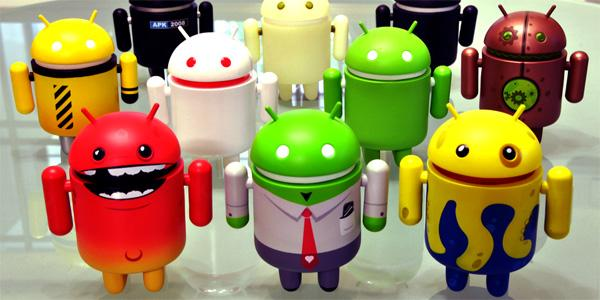
\includegraphics[scale=0.7]{img/cp05/img0503.png}

Android se creó pensando en sacarle el mayor provecho posible a los pocos recursos que puede haber en un dispositivo móvil, de esta manera sin saturar los recursos obtener los 
mejores resultados. Su arquitectura está diseñada para simplificar la reutilización de componentes; además de esto incluye un conjunto de bibliotecas de C y C++ usadas por varios 
componentes del sistema y un set de bibliotecas básicas de Java que proporciona la mayor parte de las funciones base.

Android depende de Linux para los servicios base del sistema como seguridad, gestión de memoria, gestión de procesos, pila de red y modelo de controladores. Este núcleo también 
actúa como una capa de abstracción entre el hardware y el resto de la pila de software.

Algo muy llamativo de Android, es que, al contrario de otros sistemas operativos para móviles como iOS o Windows Phone, se desarrolla de forma abierta y se puede acceder tanto al 
código fuente, como a la lista de incidencias donde se pueden ver problemas aún no resueltos y reportar problemas nuevos, de esta manera se ayuda a que cada día este software 
mejore y se adapte más a las necesidades de los usuarios.

\subsection*{CARACTERÍSTICAS}
Posee un navegador integrado basado en el motor Open Source Webkit, una base de datos llamada SQLite que permite el almacenamiento estructurado de datos y que se integra 
directamente con las aplicaciones, soporte para medios multimedia con formatos comunes de audio, video e imágenes planas como MPEG4, MP3, AAC, AMR, JPG, PNG y GIF, la base de 
llamadas de instancias se llama Dalvik y es muy similar a la máquina virtual de Java, y otras características dependientes del terminal como: tecnología GSM, EDGE, 3G, Wifi, 
Bluetooth, GPS, Cámara, Brújula y Acelerómetro.

\subsection*{ACTUALIZACIONES}
Android ha visto numerosas actualizaciones desde su liberación inicial. Estas actualizaciones al sistema operativo base típicamente arreglan bugs y agregan nuevas funciones.
Las versiones de Android reciben el nombre de postres en inglés.
\begin{itemize}
	\item \textit{Apple Pie (v1.0)}, Tarta de manzana.
	\item \textit{Banana Bread (v1.1)}, Pan de plátano.
	\item \textit{Cupcake (v1.5)}, Panque.
	\item \textit{Donut (v1.6)}, Rosquilla.
	\item \textit{Éclair (v2.0/v2.1)}, Pastel francés.
	\item \textit{Froyo (v2.2)}, Yogurt de helado.
	\item \textit{Gingerbread (v2.3)}, Pan de jengibre. 
	\item \textit{Honeycomb (v3.0/v3.1/v3.2)}, Panal de miel.
	\item \textit{Ice Cream Sandwich (v4.0)}, Sándwich de helado.
	\item \textit{Jelly Bean (v4.1/v4.2/v4.3)}, Dulces.
	\item \textit{KitKat (v4.4)}, Galleta de Chocolate.
\end{itemize}

\begin{description}
	\item[Apple Pie:]
		Lanzada el 23 de Septiembre de 2008, es considerada la más importante y la de mayor novedad en toda la evolución de Android ya que es la primera versión comercial del 
		sistema operativo y el comienzo de una nueva forma de ver los dispositivos móviles.
		
		Las características más relevantes fueron:
		\begin{itemize}
			\item Incorporación de un mercado para compra y descarga de aplicaciones bajo el nombre de Android Market.
			\item Un navegador web con soporte múltiples ventanas.
			\item Soporte básico para cámara de fotos.
			\item Posibilidad de crear carpetas e introducir iconos de aplicaciones en ellas desde el escritorio.
			\item Acceder a servidores de correo electrónico por web.
			\item Incorporación de productos de Google: GTalk, Google Maps, YouTube, Google Sync y Google Search.
			\item Sincronización con los productos de Google.
			\item Mensajería instantánea.
			\item Reproductor de música (sin soporte para reproducir vídeo).
			\item Marcación por voz.
		\end{itemize}
	
	\item[Banana Bread:]
		Lanzada el 9 Febrero de 2009 únicamente para el HTC Dream, con esta actualización se buscaba corregir algunos errores de la versión anterior, mejorar la API (Interfaz de 
		Programación de Aplicaciones) y como es normal en todas las actualizaciones, agregar nuevas características.
		
		Las características más relevantes fueron:
		\begin{itemize}
			\item Detalles y reseñas disponibles cuando un usuario busca negocios y lugares en Google Maps.
			\item Pantalla en llamada más larga por defecto cuando están en uso el manos libres.
			\item Incorporación de soporte para marquesinas en diseños de sistemas.
			\item Posibilidad de guardar archivos adjuntos en los mensajes.
			\item Posibilidad de ocultar o mostrar el teclado en pantalla.
		\end{itemize}
	
	\item[Cupcake:]
		Lanzada el 30 de abril de 2009, traía consigo mejoras muy marcadas y detalles que hacían de Android una mejor opción a la hora de escoger, con respecto a los otros sistemas 
		operativos.
		
		Las características más relevantes fueron:
		\begin{itemize}
			\item Posibilidad de subir videos a YouTube e imágenes a picaza.
			\item Grabación y reproducción en formatos MPEG-4 y 3GP.
			\item Mejoramiento de todos los principales elementos de la interfaz gráfica.
			\item Opción de auto-rotación.
			\item Pantallas de transiciones animadas.
			\item Soporte de Widgets y paquete para la pantalla de inicio, como reloj analógico, calendario, reproductor de música, marco de imágenes y búsqueda.
		\end{itemize}
	
	\item[Donut:]
		Lanzada el 15 de Septiembre 2009, incluyo nuevas características como:
		\begin{itemize}
			\item Mejora la búsqueda por voz y texto.
			\item Habilidad para ver capturas de las aplicaciones en Android Market.
			\item Mejor integración entre la galería y la cámara.
			\item Múltiple selección de imágenes para ser eliminadas.
			\item Mejoras de velocidad en aplicaciones de cámara y de búsqueda.
		\end{itemize}
		
	\item[Éclair:]
		Lanzada el 26 de Octubre de 2009, añadió nuevas mejoras como:
		\begin{itemize}
			\item Nueva interfaz de usuario.
			\item Optimización de la velocidad del hardware.
			\item Diseño mejorado de la lista de contactos.
			\item Zoom digital.
			\item Teclado virtual mejorado.
			\item Soporte para flash.
		\end{itemize}
	
	\item[Froyo:]
		Lanzada el 20 de Mayo de 2010, cuyo objetivo era mejorar el rendimiento y la memoria general del sistema, durante todo el año corrigieron errores que se presentaron.
 
		Las características más relevantes fueron:
		\begin{itemize}
			\item Mejora en la velocidad de las aplicaciones.
			\item Lanzador de aplicaciones mejorado, con accesos directos.
			\item Actualización del Android Market, con actualizaciones automáticas.
			\item Compartir contactos por Bluetooth.
			\item Opción para desactivar el tráfico de datos.
		\end{itemize}
	
	\item[Gingerbread:]
		Lanzado el 6 de Diciembre de 2010, traía consigo mejoras como:
		\begin{itemize}
			\item Administrador de descargas para descargas grandes.
			\item Soporte para pantallas con mayor resolución.
			\item Recolección de elementos recurrentes para un mayor rendimiento.
			\item Nueva interfaz de usuario.
		\end{itemize}
	
	\item[HoneyComb:]
		Lanzado el 22 de Febrero de 2011, con características como:
		\begin{itemize}
			\item Mejora en el sistema multitarea.
			\item Soporte para Widgets 3D rediseñados.
			\item Soporte para video chat mediante Google Talk.
		\end{itemize}
		
	\item[Ice Cream Sandwich:]
		 Lanzado el 19 de Octubre de 2011, en esta actualización se busca unificar el uso de cualquier dispositivo con Android.
		 
		 Las características más relevantes fueron:
		 \begin{itemize}
		 	\item Sistema multitarea mejorado.
		 	\item Interfaz mejorada, más moderna.
		 	\item Corrector de texto mejorado.
		 	\item Captura de pantalla al oprimir dos botones.
		 	\item Reconocimiento de voz.
		 \end{itemize}
		
	\item[Jelly Bean:]
		 Lanzado el 9 de Julio de 2012 y actualizado el 13 de noviembre de 2013, su objetivo principal era el de mejorar la experiencia del usuario, mejorando la funcionalidad y 
		 rendimiento de la interfaz gráfica.
 
		 Las características más relevantes fueron:
		 \begin{itemize}
		 	\item Mayor fluidez y estabilidad.
		 	\item Google Chrome como navegador por defecto.
		 	\item Notificaciones mejoradas, con acceso más rápido a la información.
		 	\item Ajuste automático en los Widgets.
		 	\item Dictado por voz mejorado.
		 	\item Creación de un modo para discapacitados visualmente, llamado Getual Mode.
		 	\item Nueva barra de búsqueda.
		 \end{itemize}
	
	\item[KitKat:]
		lanzado el 5 de noviembre de 2013 y actualizado durante el 2014, su objetivo fundamental era mejorar el rendimiento y que esta versión pudiera ser también compatible con 
		dispositivos de gama baja.  
 
		Las mejoras más significativas son:
		\begin{itemize}
			\item Modificaciones en la forma como se hacen y reciben llamadas.
			\item Solucionando la fragmentación entre versiones, corre en cualquier dispositivo, al necesitar solamente 512 MB de memoria RAM para su funcionamiento.
			\item Impresión de documentos por Wi-Fi.
			\item Reduce el consumo de batería.
			\item Mejoras en el NFC.
			\item Detector y contador de pasos.
			\item Grabación de pantalla.
		\end{itemize}
\end{description}

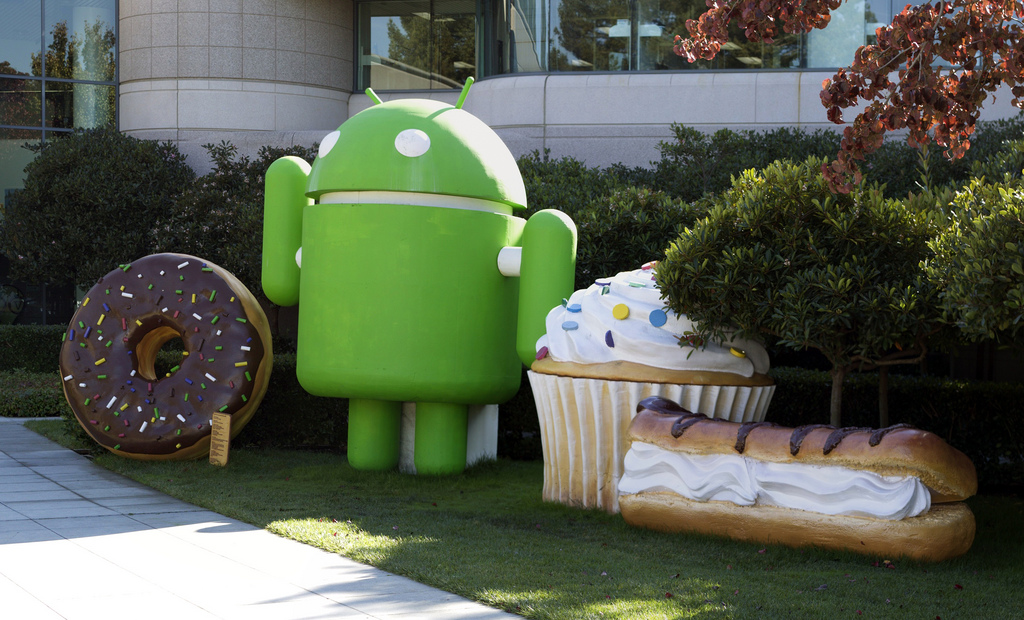
\includegraphics[scale=0.5]{img/cp05/img0504.png}

\subsection*{VENTAJAS:}
\begin{itemize}
	\item El código es Abierto; gracias a esto cualquier persona puede realizar una aplicación para Android.
	\item Hoy en Día hay más de 100,000 aplicaciones disponibles para teléfonos Android, gran parte de ellas gratuitas.
	\item Android es multitarea; es capaz de hacer funcionar a la vez varias aplicaciones.
	\item Android se puede modificar a tu gusto; puedes personalizar totalmente la pantalla.
\end{itemize} 

\subsection*{DESVENTAJAS:}
\begin{itemize}
	\item Android es multitarea; no siempre cierra todas las aplicaciones así que hace falta tener una aplicación que cierre las apps abiertas.
	\item Duración de la Batería; se gasta rápidamente.
	\item Android es poco intuitivo; problema provocado por la interfaz.
	\item Android está desfragmentado; cada modelo de teléfono móvil se ha de adaptar a Android por lo que no es la misma versión.
\end{itemize}

\subsection*{QUE HACE MEJOR:}
\begin{itemize}
	\item Android destaca por dejar cierta sensación de libertad al consumidor.
	\item Permite adaptar más la tableta a sus gustos y hacer de ella un traje a medida.
	\item Otra ventaja son los Widgets, pequeñas ventajas que muestran la información directamente en el escritorio.
	\item Los fabricantes de aparatos para Android juegan con un mayor margen creativo.
\end{itemize}


\section*{APLICACIONES ANDROID}
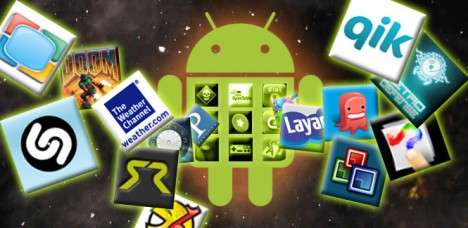
\includegraphics[scale=0.5]{img/cp05/img0505.png}

Desde que los Smartphones empezaron a entrar en furor y Android se convirtió en el sistema operativo predilecto por la mayoría de los usuarios, en general, las compañías de todo 
tipo, se vieron en la necesidad de producir aplicaciones para dispositivos móviles, evitando así quedar obsoletos. A raíz de esto es que podemos ver aplicaciones de todo tipo, 
desde juegos hasta herramientas útiles para el fomento de la educación sin importar el área.
 
Para Android existen miles de aplicaciones, la gran mayoría de estas para descargar desde la Play Store, allí encontramos aplicaciones para casi cualquier cosa y de temas 
completamente variados, muchas de estas gratuitas y otras de pago. Android también hace su aporte a la educación, teniendo disponibles muchos aplicativos al fomento de la 
educación y para facilitar el aprendizaje, como graficadores matemáticos, gestores de tareas, traductores y diccionarios, lectores de noticias, libros digitales, juegos 
educativos, etc.
 
En el ámbito matemático y científico, contamos con una gran variedad de utilidades como solucionador de ecuaciones, cálculos de expresiones algebraicas, tabla periódica de los 
elementos químicos.
 
Algunas de estas aplicaciones son:
\begin{description}
	\item[MathWay:] 
		Es una aplicación online que permite realizar operaciones matemáticas, como calculo integral o diferencial, geometría analítica, matemáticas básicas. Etc. Es una 	
		herramienta de mucha ayuda para las personas que están en constante interacción con las matemáticas y que para su trabajo o estudio, requieren poder hacer cálculos 
		especiales de manera más rápida.
	
	\item[HandyCalc:]
		Es una calculadora que permite graficar funciones, resolver operaciones trigonométricas, realizar conversiones de moneda y de unidades, resuelve funciones exponenciales y 
		aritméticas, ayuda con la sintaxis para que no se produzcan errores, en general es una calculadora muy completa y fácil de usar.
	
	\item[Solution Calculator:]
		Es una aplicación que permite hacer cálculos con soluciones químicas, es muy útil para los estudiantes de química y biología, también calcula el peso molecular de los 		
		elementos químicos, su idioma de funcionamiento es el inglés pero es muy sencillo de usar.
		
	\item[Anatomy 3D:]
		Es una aplicación que ayuda a entender de manera más didáctica la anatomía del cuerpo humano, las animaciones son en 3D y permite mover, rotar y quitar cualquier estructura 
		anatómica; es muy práctico para los estudiantes de la rama de la salud.
\end{description}

En la sección de juegos, también contamos con unas aplicaciones especiales que son los juegos educativos, algo que abunda en este sistema operativo y que nos permitirá 
desarrollar nuestro intelecto de forma más didáctica.
 
Algunos de los juegos más populares son:
\begin{description}
	\item[Preschool Adventure:]
		Es una aplicación que está compuesta por varios componentes que potencializaran el intelecto de los niños, como lo son el diferenciar sonidos, formas, colores, partes del 
		cuerpo etc, todo esto de manera muy lúdica.
		
	\item[Holoholo:]
		Es una aplicación bastante llamativa ya que permite conocer ciudades del mundo y tener la oportunidad de interactuar con algunas personas para poder resolver acertijos y 
		cumplir el objetivo del juego. Son varias historias donde el jugador deberá cumplir con los objetivos que se le asignen. Desarrolla la habilidad y el ingenio.
	
	\item[Tangram:]
		Es un juego antiguo chino que significa, la tabla de la sabiduría, consiste en armar un rompecabezas con una figura en el fondo con siete fichas (figuras geométricas) las 	
		cuales no pueden superponerse. Cada ficha se llama "tans". Con este juego se desarrolla la concentración, la observación y la capacidad espacial. Hasta el momento cuenta 
		con más de 100 rompecabezas y en cada actualización se añaden más.
	
	\item[Brain Games:]
		Es una aplicación que consta de 5 atractivos juegos mentales, en los cuales se puede entrenar el cerebro en agilidad mental, lógica matemática, visión lateral, capacidad de 
		retentiva, memorización; también permite jugar contra reloj y mejorar cada vez su propio record.
	
	\item[Trivial Gems:]
		Es uno de los mejores juegos que hay de preguntas y respuestas en Android, ya que permite jugarse hasta con 4 jugadores online, dos modos de juego y más de seis mil 
		preguntas de casi todos los temas como deportes, historia, literatura, música, etc.
\end{description}

En el área de los idiomas, podemos ver que por la necesidad de interactuar con diferentes idiomas ya sea por un saber adicional, por gusto o por necesidad del trabajo o del 
estudio, se hace cada vez más necesario que la forma en cómo se aprende un idioma extranjero sea cada vez más fácil, interactiva y de acceso más inmediato al usuario
 
Algunos de los aplicativos más utilizados para esta este aprendizaje son:
\begin{description}
	\item[Babbel:]
		Es un sistema de aprendizaje integrado que permite a las personas aprender idiomas fácilmente gracias a su sistema integrado que combina métodos pedagógicos con la 
		tecnología.

		Esta aplicación cuenta con 13 idiomas y una forma muy práctica de hacer que el usuario aprenda en poco tiempo ya que le permite realizar ejercicios de gramática, y 	
		pronunciación, así como aprender muchas más palabras y llegar a tener así, un mejor vocabulario.
	
	\item[Busuu:]
		Es una comunidad online que tiene su aplicación, en la cual puedes aprender distintos idiomas, como francés, alemán, ruso, inglés, italiano, etc. De forma más práctica, 
		divertida y natural ya que cuenta con 40 millones de hablantes nativos. Fue catalogada como la mejor App (Aplicación) gratuita del 2013 para el aprendizaje de idiomas.
		
	\item[Duolingo:]
		Es un sitio web de una empresa, que como muchas también cuenta con su aplicación para Android, y además de eso es gratuita. En Duolingo avanzan completando unidades, ganas 
		puntos por tus respuestas correctas pero también pierdes puntos con las respuestas incorrectas, vas escalando niveles como en un juego; en general es muy práctica de usar y 
		cambia la forma en que la persona aprende un idioma.
\end{description}

La forma en cómo se veía la vida ha cambiado con el surgir de las nuevas tecnologías, ahora todo es electrónico, para con esto optimizar muchas tareas. Los libros usualmente se 
tenían en físico, pero con la posibilidad de tenerlos en nuestros dispositivos móviles, esto ha quedado atrás, ya no tenemos que cargar con cientos de libros pesados, puesto que 
podemos tener la cantidad de libros que la memoria de nuestro dispositivo soporte y lo mejor aún sin talar tantos árboles.
 
Entre los lectores de libros electrónicos más usados, tenemos:
\begin{description}
	\item[Aldiko Book Reader:]
		Es una aplicación totalmente personalizable a la hora de las preferencias que tengamos para leer un libro, permite desde cambiar el tipo y tamaño de fuente, hasta el hecho 
		de poder tener marcadores, subrayar palabras claves y movernos por todo el libro de manera más fácil gracias a su buscador de páginas.
		
	\item[Kindle:]
		Este lector de libros electrónicos cuenta con una interfaz sencilla y fácil de usar, tiene acceso a más de 1.500.000 libros de los cuales hay más de 1.400 gratis. Tiene una 
		característica muy particular y es el hecho de poder buscar el significado de alguna palabra que no se tiene idea y se pueden realizar búsquedas internas en el libro, 
		también tiene caracterizas de lectura personalizada como cambiar el tamaño de la letra, cambiar el color entre otras ya mencionadas.
\end{description}

\section*{¡IMPACTANDO DESDE SU INICIO!}
Desde su lanzamiento, Android se ha posicionado como uno de los mejores sistemas operativos en cuanto a dispositivos móviles se refiere; su impacto se debe a que propone una 
forma muy novedosa de manejar muchos aspectos de nuestra vida y realizar diferentes tipos de acciones a través de nuestros Smartphones y Tablets; además el hecho de poder estar 
en contacto con el resto del mundo, se convirtió casi que en algo de primera necesidad.
 
Android, al ser de código abierto, le da carta abierta a los desarrolladores para que modifiquen y generen nuevas plataformas con vistas personalizadas; además la gran cantidad 
de aplicaciones que se encuentran disponibles en la Play Store, nos da la oportunidad de poder escoger entre muchas del mismo tipo, la que más nos guste y tener variedad entre 
juegos o herramientas útiles que nos ayudaran con algunas de nuestras tareas diarias o simplemente divertirnos.
 
El éxito de Android se puede apreciar analizando el crecimiento que ha tenido en el número de usuarios adscritos a este sistema operativo, desde su lanzamiento hasta la fecha. 
Examinando las estadísticas, podemos ver que en 2008 tras finalizar su primer año de vida contaba con un 0.5\% de los usuarios totales, en 2009 aumento a un 3.9\%, en 2010 un muy 
favorable 22.6\% que auguraba un buen futuro para este sistema operativo, en 2011 tuvo un aumento realmente significativo para llevar solo 4 años en el mercado, alcanzando una 
cifra muy alentadora para Google de un 42.0\%, en 2012 logro obtener la mitad de los usuarios del mundo con un 49.9\%, en 2013 Android ya era todo un éxito a nivel mundial y 
había roto cualquier esquema y llego a una cifra tal vez nunca antes imaginada de un 79\% de usuarios, pero en lo que llevamos de 2014 se ha venido presentando una baja, algo que 
no habíamos visto estos 6 años y que probablemente se deba al lanzamiento del iPhone 5c con su nuevo diseño renovado y a que este producto de Apple presenta menos ataques virales 
que Android.